\chapter{Implementation, Integration and Test Plan}
The implementation, integration and testing of the system will follow a bottom-up approach, without omitting the dependencies between components within the same subsystem. This approach is chosen both for the server side and the client side, that will be implemented and tested in parallel. An incremental integration facilitates bug tracking and generates working software quickly during the software life cycle.\newline
External services do not need to be unit tested since it is assumed that they are reliable.

\section{Plan Definition}
What is described below is the implementation plan of the server-side, as it is the most complex part which presents the most critical parts of the system.\newline
Please note that the client-side will be implemented and tested in parallel with the server development. The various client applications will therefore be integrated in the final diagram to show the system as a whole.

In the first step (\clupautoref{fig:bottom_up_1}) the Model and the EntityManager are implemented and unit tested using a driver for the components that are still under implementation. These components are responsible for all the interactions with the database and are needed by the majority of all the other components.
\begin{figure}[H]
	\centering
	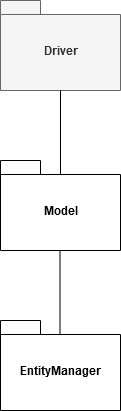
\includegraphics[width=0.12\linewidth]{bottom_up/bottom_up_1}
	\caption{Bottom-up approach first step.}
	\label{fig:bottom_up_1}
\end{figure}

In the second step (\clupautoref{fig:bottom_up_2}) the components responsible for the authentication are implemented. A stub is introduced to simulate the MailManager component. This is to give priority to the access and permissions mechanism of the system, required by other components.
\begin{figure}[H]
	\centering
	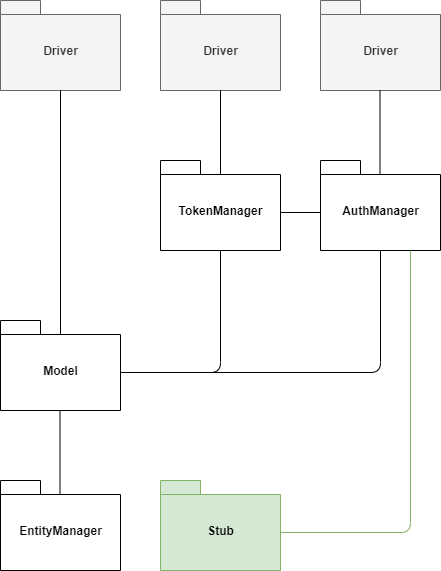
\includegraphics[width=0.5\linewidth]{bottom_up/bottom_up_2}
	\caption{Bottom-up approach second step.}
	\label{fig:bottom_up_2}
\end{figure}


The third step (\clupautoref{fig:bottom_up_3}) shows the implementation of the DashboardManager.
\begin{figure}[H]
	\centering
	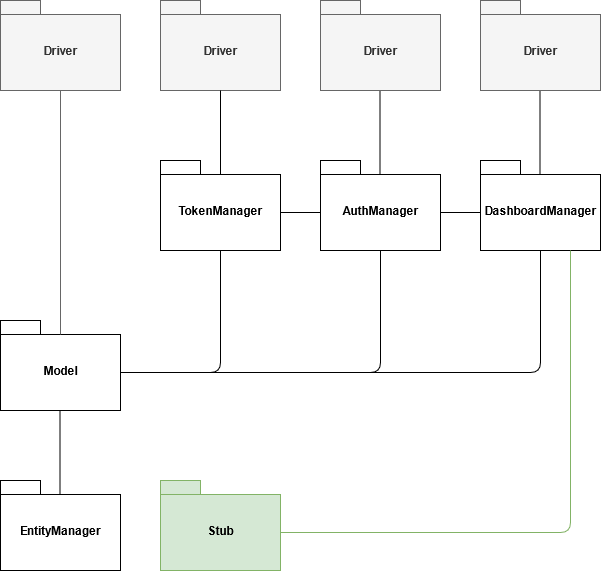
\includegraphics[width=0.5\linewidth]{bottom_up/bottom_up_3}
	\caption{Bottom-up approach third step.}
	\label{fig:bottom_up_3}
\end{figure}

In the fourth step (\clupautoref{fig:bottom_up_4}) the WebApp is integrated and supersedes the drivers for AuthManager and DashboardManager. Also the StorePassManager component is implemented and tested with its own driver.
\begin{figure}[H]
	\centering
	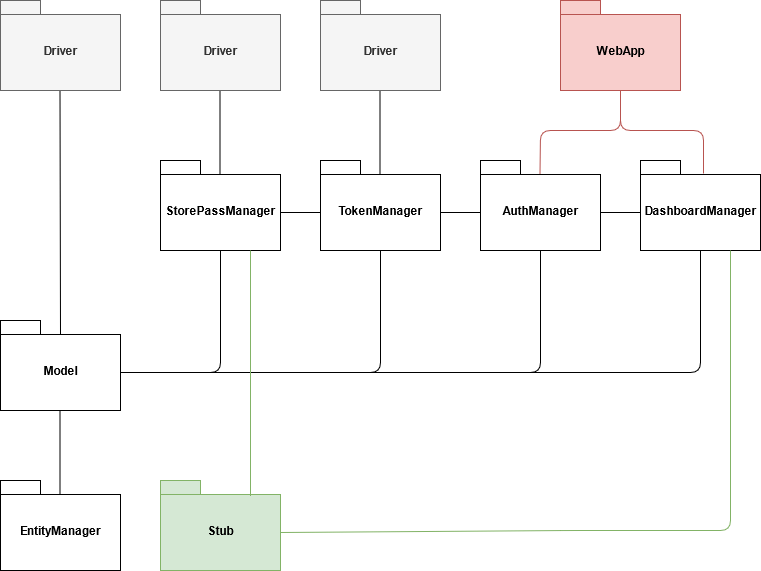
\includegraphics[width=0.95\linewidth]{bottom_up/bottom_up_4}
	\caption{Bottom-up approach fourth step.}
	\label{fig:bottom_up_4}
\end{figure}

\clearpage

The fifth step (\clupautoref{fig:bottom_up_5}) shows the implementation and testing of the remaining server components.
\begin{figure}[H]
	\centering
	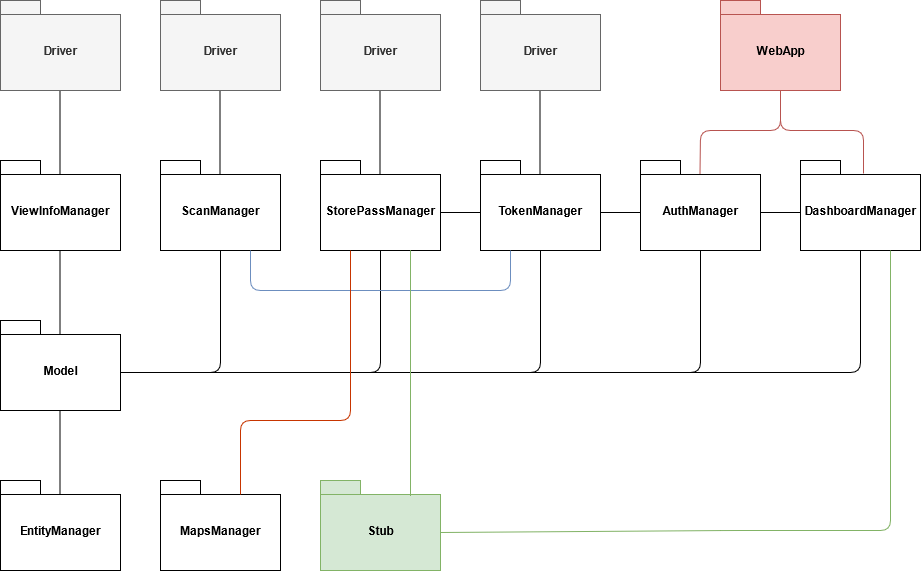
\includegraphics[width=0.95\linewidth]{bottom_up/bottom_up_5}
	\caption{Bottom-up approach fifth step.}
	\label{fig:bottom_up_5}
\end{figure}

\clearpage

The final step (\clupautoref{fig:bottom_up_6}) shows the implementation of the whole system.
\begin{figure}[H]
	\centering
	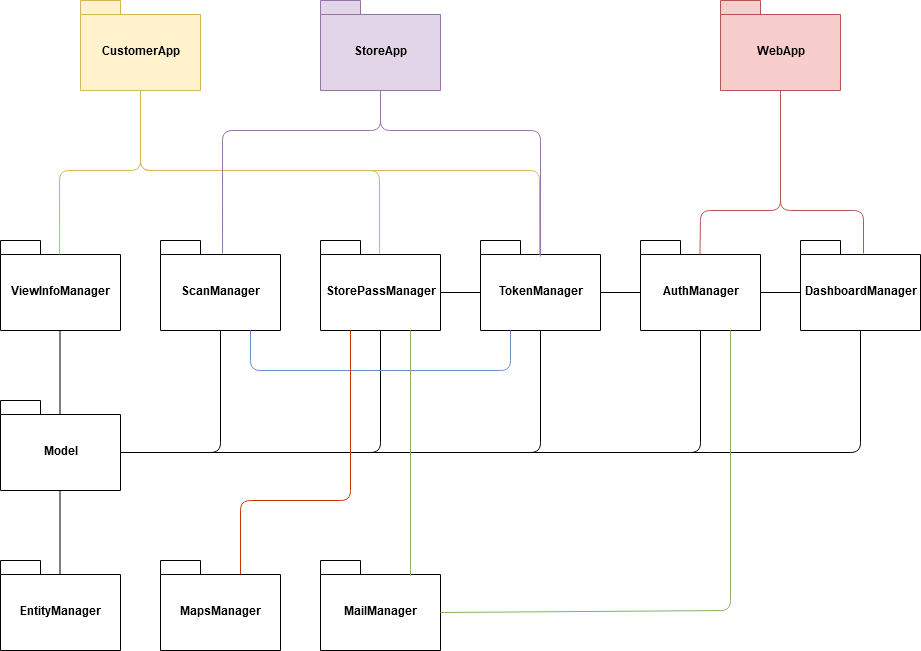
\includegraphics[width=0.95\linewidth]{bottom_up/bottom_up_6}
	\caption{Bottom-up approach final step.}
	\label{fig:bottom_up_6}
\end{figure}

\clearpage

\section{Technologies}\label{iit:tech}
This section will analyse the possible technologies available to develop each component of the system.

\subsection{Mobile}
The mobile applications must be accessible by as many users as possible, hence it must be developed for the major mobile OSes, Android and iOS.
In order to achieve this, it is possible to adopt a cross-platform development framework which  avoid the burden of having to use two different native codebases.
A lot of alternatives are available, most of them consisting of a web view, such as Apache Cordova and Ionic. 
However, for scalability and performance reasons, these options are discarded, in favour of a more native approach with Flutter, an open-source UI software development kit created by Google.
Since this framework compiles to native code, it provides better performance and scalability. A the same time, the availability of a big standard library of UI components avoids the need of third party packages which allows for faster development.

\subsection{Back-end server}
The back-end will be implemented in Java EE with the TomEE application/web server.
It allows for fast development and easy integration with documentation tools that help speed up the work.\newline
The web server will conform to the REST architectural design, providing a REST API, which allows for great flexibility.
 
\subsection{Front-end web app}
Java templating with Thymeleaf will be used for the web app interface.

\subsection{Database}
MySQL server is one of the world’s most popular databases. It is open source, reliable, cost-effective and easy to manage. For this reason, it is chosen for the data storage system.

\subsection{Token System}
For the token system the choice fell on JSON Web Token which is an internet standard.\newline
When the store employee successfully logs in using their credentials or a customer opens the app for the first time, a JSON Web Token is returned and saved locally in the app, instead of the traditional approach of creating a session in the server and returning a cookie.\newline
When the client wants to access a route the token is sent in the HTTPS request. This is a stateless authentication mechanism as the user state is never saved in server memory. The server's protected routes will check for a valid JWT in the request, and if it is present, the user will be allowed to the resources.\newline
As JWTs are self-contained, all the necessary information is there, reducing the need to query the database multiple times.

\subsection{Testing tools}
Automated tests help ensure that the applications performs correctly before publishing them, while retaining features and bug fixes velocity. Several tools are needed:
\begin{itemize}
	\item \textbf{JUnit}: a unit testing framework for the Java programming language. It allows to define the test for each of the	parts developed in a Java application. It is very well documented and allows to be integrated with other testing tools.
	
	\item The \textbf{test} and \textbf{flutter\_test} packages provided by the core Flutter framework: the \textit{test package} provides the core framework for writing unit tests for the mobile applications and the \textit{flutter\_test package} provides additional utilities for testing widgets.
	
	\item \textbf{Mockito}: a popular mock framework which can be used in conjunction with JUnit and Flutter testing packages. Mockito allows to create and configure mock objects. Using Mockito greatly simplifies the development of tests for classes with external dependencies.

\end{itemize}
